\newpage
\section{Additional \textsc{HubbleUnlearning} results}
\label{sec:unlearn_grid_search} \label{sec:unlearn_full_results}
% \subsection{Grid Search Configurations}

Below are the detailed hyperparameters for each method: 

\begin{table}[h]
\centering
\small
\setlength{\tabcolsep}{6pt}
\renewcommand{\arraystretch}{1.2}
\begin{tabular}{lccc}
\toprule
\textbf{Hyperparameter} & \textbf{RMU} & \textbf{RR} & \textbf{SatImp} \\
\midrule
\textbf{Training type} & Layer FT & LoRA FT & Full FT \\
\textbf{Layers / Targets} & 5, 6, 7 & 10, 20 (transform all) & --- \\
\textbf{LoRA Rank / $\alpha$ / Dropout} & --- & 16 / 16 / 0.05 & --- \\
\textbf{LoRRA $\alpha$} & --- & 10 & --- \\
\textbf{Alpha ($\alpha$)} & 100, 1000, 10000 & --- & 0.01, 0.1, 1 \\
\textbf{Steering coefficient} & 5, 50, 500 & --- & --- \\
\textbf{$\beta_1$, $\beta_2$} & --- & --- & (5, 6), 1 \\
\textbf{Learning rate} & 5e-5, 1e-5, 5e-4 & 5e-5, 1e-4, 5e-4, 1e-3 & 1e-5, 5e-5, 1e-4 \\
\textbf{Effective batch size} & 4 & 8 & 16 \\
\textbf{Epochs} & 4, 8 & 4, 8 & --- \\
\textbf{Sample max length} & 512 & 256 & 256 \\
\bottomrule
\end{tabular}
\caption{\textbf{Grid search configurations for unlearning methods.} Each method is tuned over the listed hyperparameters. RMU and RR involve partial fine-tuning, while SatImp uses full fine-tuning.}
\label{tab:unlearn_grid_search}
\end{table}
\clearpage

% \subsection{Full Unlearning Results}

We provide the full scale unlearning results for Gutenberg in Figure \ref{fig:appendix_unlearn_gutenberg} and YAGO in Figure \ref{fig:appendix_unlearn_yago}.


\begin{figure}[h]
  \centering
  \begin{subfigure}{.48\textwidth}
    \centering
    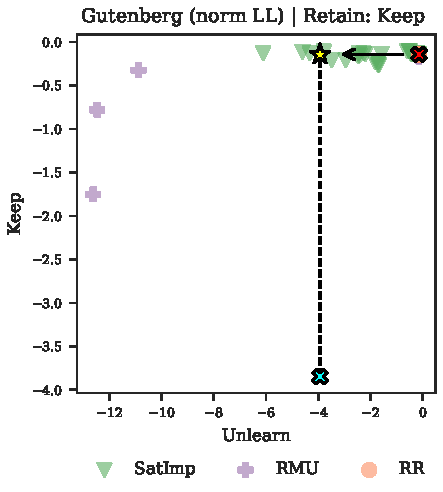
\includegraphics[width=\linewidth]{figures/Hubble_unlearn/appendix/gutenberg_keep_keep.pdf}\\[0.5em]
    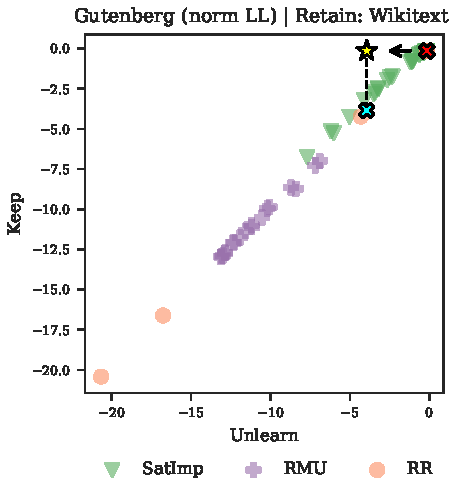
\includegraphics[width=\linewidth]{figures/Hubble_unlearn/appendix/gutenberg_wikitext_keep.pdf}
    % \caption{Gutenberg with Keep set as retain set}
  \end{subfigure}\hfill
  \begin{subfigure}{.48\textwidth}
    \centering
    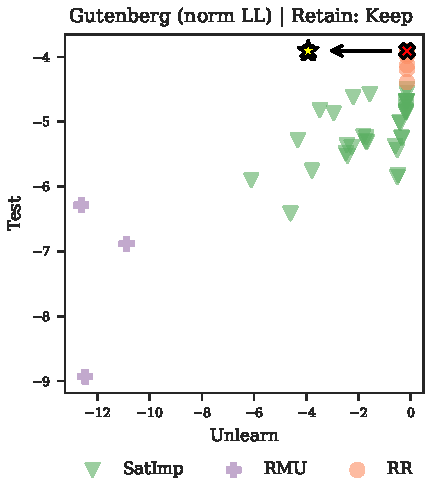
\includegraphics[width=\linewidth]{figures/Hubble_unlearn/appendix/gutenberg_keep_test.pdf}\\[0.5em]
    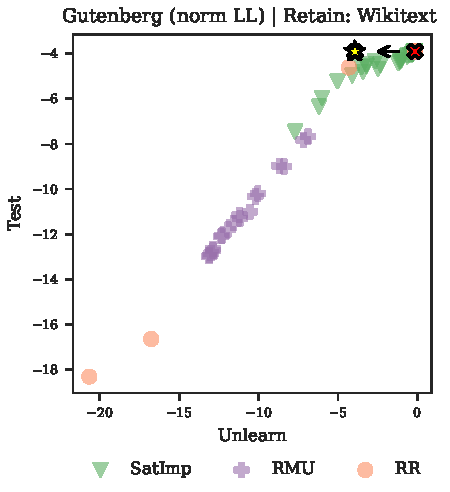
\includegraphics[width=\linewidth]{figures/Hubble_unlearn/appendix/gutenberg_wikitext_test.pdf}
    % \caption{Gutenberg with Wikitext as retain set}
  \end{subfigure}
  \caption{\textbf{Unlearning results on Gutenberg Unpopular.} Unlearning results using (out-of-domain, unseen) Wikitext (lower row) and (in-domain, seen) Keep set (upper row) as the retain sets. None of the unlearning methods simultaneously achieve the target behavior on both the seen Keep set (left column) and the unseen Test set (right column).}
  \label{fig:appendix_unlearn_gutenberg}
\end{figure}

\begin{figure}[h]
  \centering
  \begin{subfigure}{.48\textwidth}
    \centering
    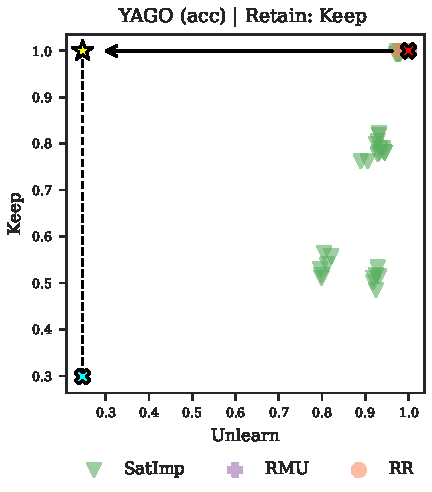
\includegraphics[width=\linewidth]{figures/Hubble_unlearn/appendix/yago_keep_keep.pdf}\\[0.5em]
    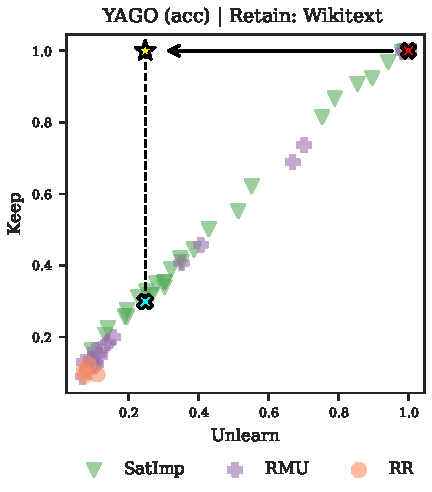
\includegraphics[width=\linewidth]{figures/Hubble_unlearn/appendix/yago_wikitext_keep.pdf}
    % \caption{YAGO with Keep set as retain set}
  \end{subfigure}\hfill
  \begin{subfigure}{.48\textwidth}
    \centering
    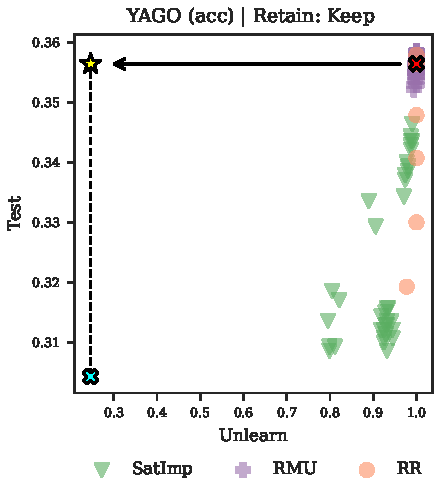
\includegraphics[width=\linewidth]{figures/Hubble_unlearn/appendix/yago_keep_test.pdf}\\[0.5em]
    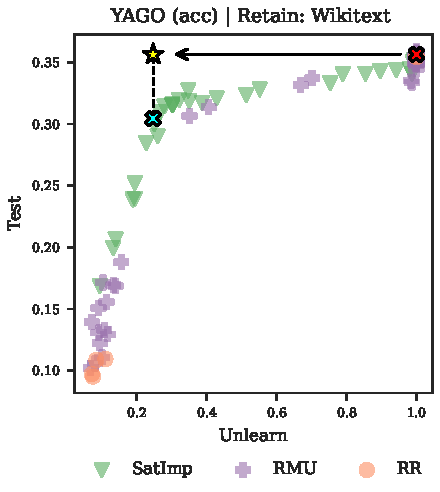
\includegraphics[width=\linewidth]{figures/Hubble_unlearn/appendix/yago_wikitext_test.pdf}
    % \caption{YAGO with Wikitext as retain set}
  \end{subfigure}
  \caption{\textbf{Unlearning results on YAGO biographies.} Unlearning results using (out-of-domain, unseen) Wikitext (lower row) and (in-domain, seen) Keep set (upper row) as the retain sets. None of the unlearning methods simultaneously achieve the target behavior on both the seen Keep set (left column) and the unseen Test set (right column).}
  \label{fig:appendix_unlearn_yago}
\end{figure}
\clearpage

% \begin{figure*}[t]
%   \centering
%   \begin{subfigure}{.48\textwidth}
%     \centering
%     \includegraphics[width=\linewidth]{figures/Hubble_unlearn/appendix/mmlu_keep_keep.pdf}\\[0.5em]
%     \includegraphics[width=\linewidth]{figures/Hubble_unlearn/appendix/mmlu_wikitext_keep.pdf}
%     \caption{MMLU with Keep set as retain set}
%   \end{subfigure}\hfill
%   \begin{subfigure}{.48\textwidth}
%     \centering
%     \includegraphics[width=\linewidth]{figures/Hubble_unlearn/appendix/mmlu_keep_test.pdf}\\[0.5em]
%     \includegraphics[width=\linewidth]{figures/Hubble_unlearn/appendix/mmlu_wikitext_test.pdf}
%     \caption{MMLU with Wikitext as retain set}
%   \end{subfigure}
%   \caption{\textbf{MMLU results.} Full unlearning results across two retain sets.}
%   \label{fig:appendix_unlearn_mmlu}
% \end{figure*}

% \paragraph{RMU \citep{wmdp}:}
% \begin{itemize}
%   \item Layer Fine-tuning:
%   \begin{itemize}
%     \item Layers: 5, 6, 7
%   \end{itemize}
%   \item Alpha: 100, 1000, 10000
%   \item Steering coefficient: 5, 50, 500
%   \item Learning rate: \texttt{5e-5}, \texttt{1e-5}, \texttt{5e-4}
%   \item Effective batch size: 4
%   \item Epochs: 4, 8
%   \item Sample max length: 512
% \end{itemize}

% \paragraph{RR \citep{rr}:}
% \begin{itemize}
%   \item LoRA Fine-tuning:
%   \begin{itemize}
%     \item LoRA Rank: 16
%     \item LoRA $\alpha$: 16
%     \item LoRA dropout: 0.05
%   \end{itemize}
%   \item LoRRA Alpha: 10
%   \item Target layers: 10, 20
%   \item Transform layers: all
%   \item Learning rate: \texttt{5e-5}, \texttt{1e-4}, \texttt{5e-4}, \texttt{1e-3}
%   \item Effective batch size: 8
%   \item Epochs: 4, 8
%   \item Sample max length: 256
% \end{itemize}

% \paragraph{SatImp \citep{satimp}:}
% \begin{itemize}
%   \item $\alpha$: 0.01, 0.1, 1
%   \item $\beta_1$: 5, 6
%   \item $\beta_2$: 1
%   \item Learning rate: \texttt{1e-5}, \texttt{5e-5}, \texttt{1e-4}
%   \item Effective batch size: 16
%   \item Sample max length: 256
% \end{itemize}

% After grid search, we evaluate the unlearned checkpoints on tinyMMLU, tinyWinogrande, and tinyHellaswag from TinyBenchmarks \citep{tinybenchmarks} for general capabilities preservation, and discard checkpoints with average performance degradation exceeding 10\%.
